% qual o tempo da apresentação? apresento os apêndices? apresento os trabalhos relacionados? apresento as referências (90)?  
%	Name			:: 	sthlm Beamer Theme  HEAVILY based on the hsrmbeamer theme (Benjamin Weiss)
%	Author			:: 	Mark Hendry Olson (mark@hendryolson.com)
%	Created			::	2013-07-31
%	Updated	    	::	[[April]] 04, 2017 at 16:26:39
%	Version			:: 	2.0.2
%	Email			:: 	hendryolson@gmail.com
%	Website			:: 	http://markolson.se
%	Twitter			:: 	markolsonse
%	Instagram		:: 	markolsonse
%
%	License			:: 	This file may be distributed and/or modified under the
%					GNU Public License.
%
%	Description		::	This presentation is a demonstration of the sthlm beamer
%					theme, which is HEAVILY based on the HSRM beamer theme created by Benjamin Weiss
%					(benjamin.weiss@student.hs-rm.de), which can be found on GitHub
%					<https://github.com/hsrmbeamertheme/hsrmbeamertheme>.  It also borrows heavily
%					from the work of Matthias Vogelgesang, (https://bloerg.net) and his Metropolis Mtheme,
%					<https://github.com/matze/mtheme>.
%
%	Theme			::	newPxFont
%	Options			::	progressbar
%					::	sectionpages
%					::	numfooter
%					::	fullfooter
%					::	dovaligncolumns
%					::	protectframetitle
%					::	greybg
%					::	cblock
%					::	minimal

%-=-=-=-=-=-=-=-=-=-=-=-=-=-=-=-=-=-=-=-=-=-=-=-=
%
%        LOADING DOCUMENT
%
%-=-=-=-=-=-=-=-=-=-=-=-=-=-=-=-=-=-=-=-=-=-=-=-=

\documentclass[newPxFont, numfooter, sectionpages]{beamer}
\usepackage[utf8]{inputenc}
\usetheme{sthlm}
\usepackage{pgfplots}
\pgfplotsset{compat=1.9}
\usepackage{cancel}
\usepackage{amsthm,amsmath}
\usepackage{mathtools}

\usepackage{booktabs}
\usepackage{supertabular}
\usepackage{tabularx}
\usepackage{longtable}
\usepackage{multirow}
\usepackage{hhline}
\usepackage{color, colortbl}

\DeclarePairedDelimiter\abs{\lvert}{\rvert}%
\DeclarePairedDelimiter\norm{\lVert}{\rVert}%
\DeclareMathOperator*{\argmin}{arg\,min}
\DeclareMathOperator*{\argmax}{arg\,max}

\definecolor{lightgray}{gray}{0.8}
\definecolor{Gray}{gray}{0.9}


\title{Discriminative Sensing Based on Signal Processing for Information Security Analysis}
\subtitle{\small{Ph.D. Thesis Qualification}}
\date{\today}
\author{\texttt{Thiago P. de B. Vieira \newline \textbf{Advisor:} João Paulo C. L. da Costa} }
\institute{Universidade de Brasília 
	\par \scriptsize{Departamento de Engenharia Elétrica - ENE/FT}
	\par \scriptsize{Progama de Pós-Graduação em Engenharia Elétrica - PPGEE}
}

\hypersetup{
	pdfauthor = {Thiago P. de B. Vieira},
	pdfsubject = {Discriminative Sensing Based on Signal Processing for Information Security Analysis},
	pdfkeywords = {Signal Processing, Information Security Analysis},
	pdfmoddate= {/home/thiago/dev/projects/discriminative-sensing/docs/thesis/slides},
	pdfcreator = {Sublime and Latex}
}

\begin{document}

%-=-=-=-=-=-=-=-=-=-=-=-=-=-=-=-=-=-=-=-=-=-=-=-=
%
%	TITLE PAGE
%
%-=-=-=-=-=-=-=-=-=-=-=-=-=-=-=-=-=-=-=-=-=-=-=-=
\maketitle
%-=-=-=-=-=-=-=-=-=-=-=-=-=-=-=-=-=-=-=-=-=-=-=-=
%	FRAME: Theme Package Requirements
%-=-=-=-=-=-=-=-=-=-=-=-=-=-=-=-=-=-=-=-=-=-=-=-=
\begingroup
\setbeamercolor{normal text}{fg=\cnDarkGrey,bg=white}


%-=-=-=-=-=-=-=-=-=-=-=-=-=-=-=-=-=-=-=-=-=-=-=-=
%
%	TABLE OF CONTENTS: OVERVIEW
%
%-=-=-=-=-=-=-=-=-=-=-=-=-=-=-=-=-=-=-=-=-=-=-=-=
\section*{Outline}
\begin{frame}{Outline}
	\tableofcontents[hideallsubsections]% For longer presentations use hideallsubsections option
\end{frame}

%-=-=-=-=-=-=-=-=-=-=-=-=-=-=-=-=-=-=-=-=-=-=-=-=
%
%	TABLE OF CONTENTS: OVERVIEW
%
%-=-=-=-=-=-=-=-=-=-=-=-=-=-=-=-=-=-=-=-=-=-=-=-=
\section{Introduction}
%-=-=-=-=-=-=-=-=-=-=-=-=-=-=-=-=-=-=-=-=-=-=-=-=
%	FRAME: Motivation
%-=-=-=-=-=-=-=-=-=-=-=-=-=-=-=-=-=-=-=-=-=-=-=-=
\begin{frame}[c]{Motivation}
	It is necessary investments to detect \textbf{novel attacks and their variations}
	\begin{itemize}
		\item Signal processing schemes have being applied to detect malicious traffic;		
	\end{itemize}
	Secure mobile cloud architecture is challenging, specially in \textbf{offline mode}
	\begin{itemize}
		\item Signal processing can be applied to \textbf{behavioral analysis of mobile apps in offline mode};		
	\end{itemize}
\end{frame}
%-=-=-=-=-=-=-=-=-=-=-=-=-=-=-=-=-=-=-=-=-=-=-=-=
%	FRAME: Motivation
%-=-=-=-=-=-=-=-=-=-=-=-=-=-=-=-=-=-=-=-=-=-=-=-=
\begin{frame}[c]{Motivation}
	\textbf{Fraud detection} of \textbf{Mobile Money Transactions} has been motivating investments
	\begin{itemize}
		\item The \textbf{extraction of relevant information} from \textbf{raw or big} data is useful for classification problems and for security analysis.;
		\item Imbalanced data is challenging for classification related to anomaly detection, novelty detection, fraud detection and attack detection;
		\item \textbf{Tensor-based} algorithms for \textbf{dictionary learning} can improve \textbf{discriminative sensing} for classification in information security analysis;
	\end{itemize}
\end{frame}
%-=-=-=-=-=-=-=-=-=-=-=-=-=-=-=-=-=-=-=-=-=-=-=-=
%	FRAME: Problem Statement
%-=-=-=-=-=-=-=-=-=-=-=-=-=-=-=-=-=-=-=-=-=-=-=-=
\begin{frame}[c]{Problem Statement}
	This thesis outlines the development and evaluation of approaches based on \textbf{signal processing for information security analysis}
	\begin{itemize}
		\item To make the data discriminative;
		\item For network attack detection, mobile malicious behavior analysis and fraud detection in mobile money transactions.
	\end{itemize}
\end{frame}
%-=-=-=-=-=-=-=-=-=-=-=-=-=-=-=-=-=-=-=-=-=-=-=-=
%	FRAME: Problem Statement
%-=-=-=-=-=-=-=-=-=-=-=-=-=-=-=-=-=-=-=-=-=-=-=-=
\begin{frame}[c]{Problem Statement}
	We propose an approach based on \textbf{signal processing techniques for detection of malicious traffic in computer networks}
	\begin{itemize}
		\item Signal processing formulation as legitimate traffic, malicious traffic and noise;
		\item MOS and eigenvalue analysis are applied to detect time frames under attack;
		\item Eigen similarity analysis for extracting detailed information about accurate time and network ports under attack;
		\item Accuracy and performance evaluation through experimental scenario and the DARPA 1998 dataset.
	\end{itemize}
\end{frame}
%-=-=-=-=-=-=-=-=-=-=-=-=-=-=-=-=-=-=-=-=-=-=-=-=
%	FRAME: Problem Statement
%-=-=-=-=-=-=-=-=-=-=-=-=-=-=-=-=-=-=-=-=-=-=-=-=
\begin{frame}[c]{Problem Statement}
	This thesis also proposes an \textbf{architecture and approach based on user behavior analysis of mobile apps}
	\begin{itemize}
		\item An architecture for mobile security analysis;
		\item Offline user behavior analysis based on MOS;
		\item Scenario analysis for feature selection;
		\item Processing time evaluation in mobile devices.
	\end{itemize}
\end{frame}
%-=-=-=-=-=-=-=-=-=-=-=-=-=-=-=-=-=-=-=-=-=-=-=-=
%	FRAME: Problem Statement
%-=-=-=-=-=-=-=-=-=-=-=-=-=-=-=-=-=-=-=-=-=-=-=-=
\begin{frame}[c]{Problem Statement}
	We also propose a \textbf{tensor-based dictionary learning method for fraud detection from imbalanced data}, in order to apply the tensor decomposition for dictionary learning methods to evidentiate the \textbf{discriminative sensing of a fraud detection dataset}
	\begin{itemize}
		\item A sparse representation based classification (SRC) method through learning a tensor-based dictionary;
		\item Apply the learned dictionaries to reconstruct a test signal and classify it as fraud or legitimate;
		\item Evaluate the reconstruction error for fraud classification of mobile money transactions.
	\end{itemize}
\end{frame}
%-=-=-=-=-=-=-=-=-=-=-=-=-=-=-=-=-=-=-=-=-=-=-=-=
%	FRAME: Contributions
%-=-=-=-=-=-=-=-=-=-=-=-=-=-=-=-=-=-=-=-=-=-=-=-=
\begin{frame}{Contributions}
	\begin{enumerate}
		\item An approach based on \textbf{eigen similarity analysis} for extracting detailed information about accurate time and network ports under network attack;
		\item Computational \textbf{complexity analysis} of the proposed framework;
		\item An architecture and techniques for \textbf{offline behavioral analysis} of a corporate mobile client security architecture;
		\item A \textbf{tensor-based dictionary learning} approach for \textbf{fraud detection} in mobile payment transactions;
	\end{enumerate}
\end{frame}


%-=-=-=-=-=-=-=-=-=-=-=-=-=-=-=-=-=-=-=-=-=-=-=-=
%
%	SECTION: Model Order Selection and Eigen Similarity based Framework for Detection and Identification of Network Attacks
%
%-=-=-=-=-=-=-=-=-=-=-=-=-=-=-=-=-=-=-=-=-=-=-=-=
\section{Model Order Selection and Eigen Similarity based Framework for Detection and Identification of Network Attacks}
%-=-=-=-=-=-=-=-=-=-=-=-=-=-=-=-=-=-=-=-=-=-=-=-=
%	FRAME: Introduction
%-=-=-=-=-=-=-=-=-=-=-=-=-=-=-=-=-=-=-=-=-=-=-=-=
\begin{frame}[c]{Introduction}
	We model the network traffic as a signal processing formulation (\textbf{legitimate traffic, malicious traffic and noise})
	\begin{itemize}
		\item The proposed technique is based on eigenvalue analysis, model order selection (MOS) and similarity analysis;
		\item MOS and eigenvalue analysis are applied to detect time frames under attack;
		\item Eigen similarity analysis for extracting detailed time and network ports under attack. 
	\end{itemize}
\end{frame}
%-=-=-=-=-=-=-=-=-=-=-=-=-=-=-=-=-=-=-=-=-=-=-=-=
%	FRAME: Introduction
%-=-=-=-=-=-=-=-=-=-=-=-=-=-=-=-=-=-=-=-=-=-=-=-=
\begin{frame}[c]{Introduction}
	We model the network traffic as a signal processing formulation (\textbf{legitimate traffic, malicious traffic and noise})
	\begin{itemize}
		\item The proposed technique is based on eigenvalue analysis, model order selection (MOS) and similarity analysis;
		\item MOS and eigenvalue analysis are applied to detect time frames under attack;
		\item Eigen similarity analysis for extracting detailed time and network ports under attack. 
	\end{itemize}
\end{frame}
%-=-=-=-=-=-=-=-=-=-=-=-=-=-=-=-=-=-=-=-=-=-=-=-=
%	FRAME: Related works
%-=-=-=-=-=-=-=-=-=-=-=-=-=-=-=-=-=-=-=-=-=-=-=-=
\begin{frame}[c]{Related works}
	
	Classical methods typically employ data mining [39, 34, 70] and regular file analysis [76] to detect patterns that indicate the presence of specific attacks in network traffic;

	Callegari \emph{et al} [104] propose a PCA-based method for identifying the traffic flows responsible for an anomaly detected at the aggregate level and evaluated their proposal through a dataset with synthetic anomalies added in the data. However, Callegari \emph{et al} focus on flood attack detection, not addressing probe attack detection, and their approach relies on visual analysis. 

\end{frame}
%-=-=-=-=-=-=-=-=-=-=-=-=-=-=-=-=-=-=-=-=-=-=-=-=
%	FRAME: Related works
%-=-=-=-=-=-=-=-=-=-=-=-=-=-=-=-=-=-=-=-=-=-=-=-=
\begin{frame}[c]{Related works}
	
	Lee \emph{et al.} [61] propose OverSampling PCA (osPCA), determines the anomaly of the target according to the variation of eigenvector by similarity analysis and over sampling. In contrast, we apply MOS for detection of time frames under attack and similarity analysis to extract details for detection of time and ports under attack, for flood and probe attacks;

	Lu and Ghorbani [63] proposed a network anomaly detection model based on network flow, wavelet approximation, and system identification theory. However, their work requires a training method and presents limitations on identification of behaviors without significant outliers;

	Zonglin \emph{et al} [104] proposed a method to detect traffic anomaly with correlation analysis, but the work is not applied to probe and flood attack detection. 

\end{frame}
%-=-=-=-=-=-=-=-=-=-=-=-=-=-=-=-=-=-=-=-=-=-=-=-=
%	FRAME: Data Model
%-=-=-=-=-=-=-=-=-=-=-=-=-=-=-=-=-=-=-=-=-=-=-=-=
\begin{frame}{Data Model}
	
	Focus on \textbf{probe} and \textbf{flooding} attacks;

	Two scenarios: A \textbf{synthetic dataset} as a signal superposition of legitimate traffic, noise and malicious traffic, and selected cases of \textbf{DARPA dataset} that reproduce probe and flooding attacks.

\end{frame}
%-=-=-=-=-=-=-=-=-=-=-=-=-=-=-=-=-=-=-=-=-=-=-=-=
%	FRAME: Data Model
%-=-=-=-=-=-=-=-=-=-=-=-=-=-=-=-=-=-=-=-=-=-=-=-=
\begin{frame}{Data Model}
	
	Network traffic:

	\begin{equation}\label{eq:eq01}
		\boldsymbol{X}^{(q)} = \boldsymbol{U}^{(q)} + \boldsymbol{N}^{(q)} + \boldsymbol{A}^{(q)},
	\end{equation}

	$\boldsymbol{X}^{(q)} \in \mathbb{R}^{M \times N}$ has \emph{M} rows and \emph{N} columns. 

	Each row is a TCP or UDP port, and each column represents time bins (minute)

	Each element $x_{m,n}^{(q)}$ stands for the number of times that the port $m$ appears at the $n$-th minute, at the $q$-th time frame.

\end{frame}
%-=-=-=-=-=-=-=-=-=-=-=-=-=-=-=-=-=-=-=-=-=-=-=-=
%	FRAME: Synthetic Dataset
%-=-=-=-=-=-=-=-=-=-=-=-=-=-=-=-=-=-=-=-=-=-=-=-=
\begin{frame}[c]{Synthetic Dataset}
	
	\begin{figure}[h!]
	     \centering
	     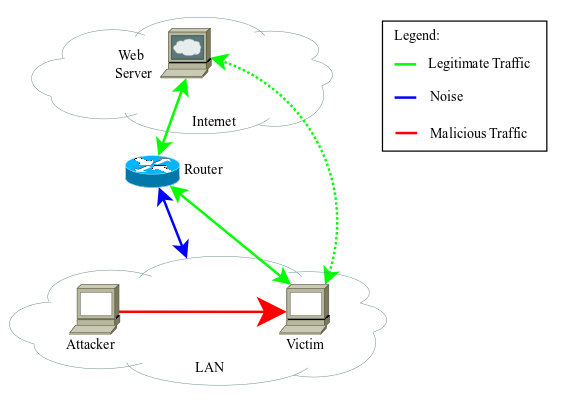
\includegraphics[width=9cm]{../figures/fig09.png}
	     \caption{Scenario to reproduce legitimate traffic, noise, flood and port scan.}
	     \label{fig:2_fig1}
	\end{figure}

\end{frame}
%-=-=-=-=-=-=-=-=-=-=-=-=-=-=-=-=-=-=-=-=-=-=-=-=
%	FRAME: Synthetic Dataset
%-=-=-=-=-=-=-=-=-=-=-=-=-=-=-=-=-=-=-=-=-=-=-=-=
\begin{frame}[c]{Synthetic Dataset}
	
	\begin{figure}[h!]
	     \centering 
	     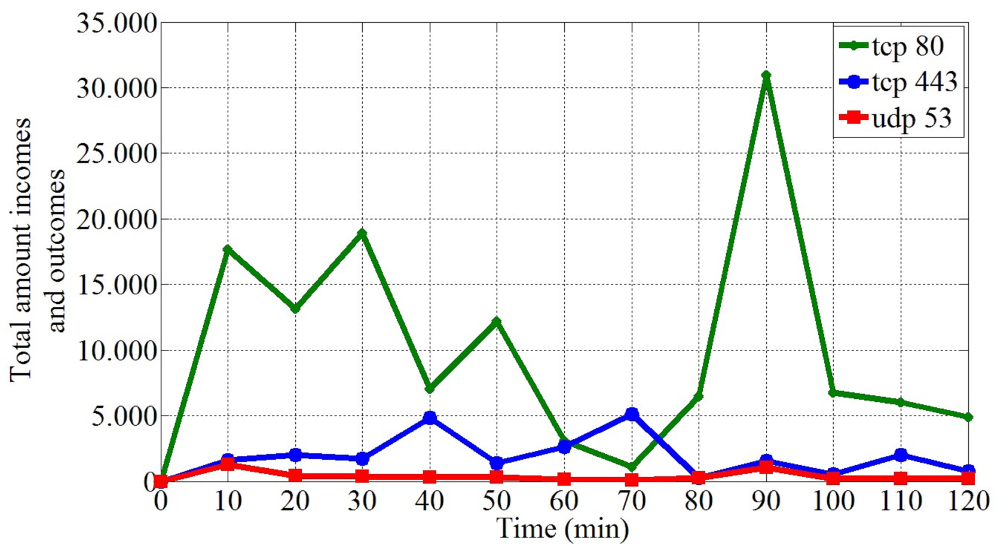
\includegraphics[width=9cm]{../figures/fig03.png}
	     \caption{Traffic from user's operations, that can be characterized by web access, traffic of well-known applications or network protocols.}
	     \label{fig:2_fig3}
	\end{figure}

\end{frame}
%-=-=-=-=-=-=-=-=-=-=-=-=-=-=-=-=-=-=-=-=-=-=-=-=
%	FRAME: Synthetic Dataset
%-=-=-=-=-=-=-=-=-=-=-=-=-=-=-=-=-=-=-=-=-=-=-=-=
\begin{frame}[c]{Synthetic Dataset}
	
	\begin{figure}[h!]
	     \centering 
	     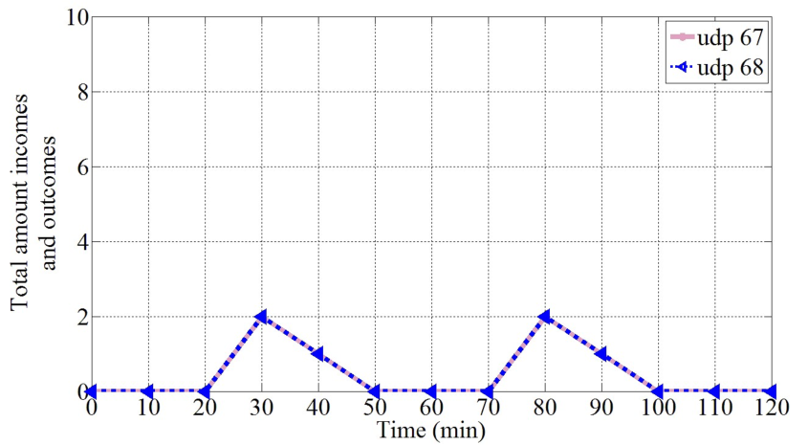
\includegraphics[width=9cm]{../figures/fig04.png}
	     \caption{Network traffic of user independent operations for network management.}
	     \label{fig:2_fig4}
	\end{figure}

\end{frame}
%-=-=-=-=-=-=-=-=-=-=-=-=-=-=-=-=-=-=-=-=-=-=-=-=
%	FRAME: Synthetic Dataset
%-=-=-=-=-=-=-=-=-=-=-=-=-=-=-=-=-=-=-=-=-=-=-=-=
\begin{frame}[c]{Synthetic Dataset}
	
	\begin{figure}[h!]
	     \centering 
	     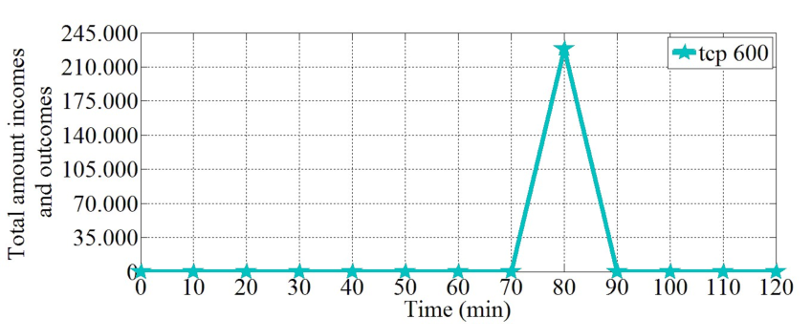
\includegraphics[width=9cm]{../figures/fig05.png}
	     \caption{A large quantity of SYN requests to a target, in order to cause a DoS.}
	     \label{fig:2_fig5}
	\end{figure}

\end{frame}
%-=-=-=-=-=-=-=-=-=-=-=-=-=-=-=-=-=-=-=-=-=-=-=-=
%	FRAME: Synthetic Dataset
%-=-=-=-=-=-=-=-=-=-=-=-=-=-=-=-=-=-=-=-=-=-=-=-=
\begin{frame}[c]{Synthetic Dataset}
	
	\begin{figure}[h!]
	     \centering 
	     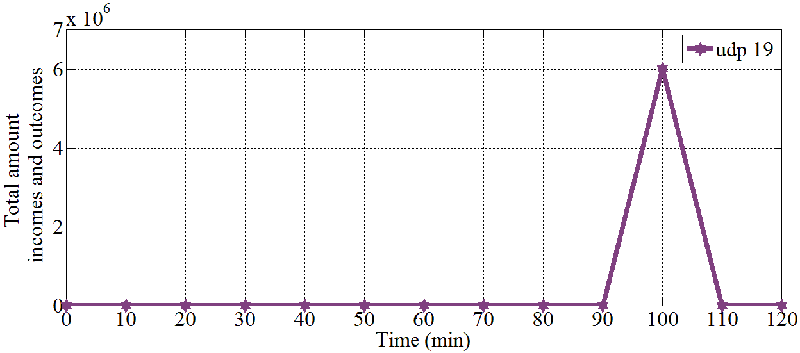
\includegraphics[width=9cm]{../figures/fig06.png}
	     \caption{Large amount of “UDP echo” requests and replies, causing packet flooding.}
	     \label{fig:2_fig6}
	\end{figure}

\end{frame}
%-=-=-=-=-=-=-=-=-=-=-=-=-=-=-=-=-=-=-=-=-=-=-=-=
%	FRAME: Synthetic Dataset
%-=-=-=-=-=-=-=-=-=-=-=-=-=-=-=-=-=-=-=-=-=-=-=-=
\begin{frame}[c]{Synthetic Dataset}
	
	\begin{figure}[h!]
	     \centering 
	     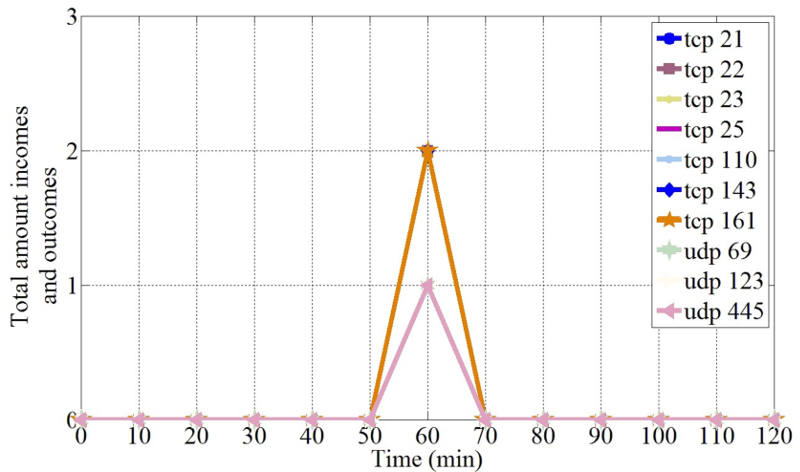
\includegraphics[width=9cm]{../figures/fig07.png}
	     \caption{Connection attempts in order to identify active ports.}
	     \label{fig:2_fig7}
	\end{figure}

\end{frame}
%-=-=-=-=-=-=-=-=-=-=-=-=-=-=-=-=-=-=-=-=-=-=-=-=
%	FRAME: DARPA Dataset
%-=-=-=-=-=-=-=-=-=-=-=-=-=-=-=-=-=-=-=-=-=-=-=-=
\begin{frame}{DARPA Dataset}
	
	7 weeks of sniffed traffic saved into raw TCPDUMP packet data, from inside and outside origins, with labeled attacks. 

	The attacks in this dataset can be grouped into: denial-of-service (DoS); remote to local (R2L); user to root (U2R); and probe attack. 

	The most cases of DoS focus on exploit system vulnerabilities instead of on flooding attack. 

	We select the cases that reproduce probe and flooding attacks.

\end{frame}
%-=-=-=-=-=-=-=-=-=-=-=-=-=-=-=-=-=-=-=-=-=-=-=-=
%	FRAME: Proposed Framework
%-=-=-=-=-=-=-=-=-=-=-=-=-=-=-=-=-=-=-=-=-=-=-=-=
\begin{frame}{Proposed Framework}
	
	\begin{figure}[h!]
		\centering
	     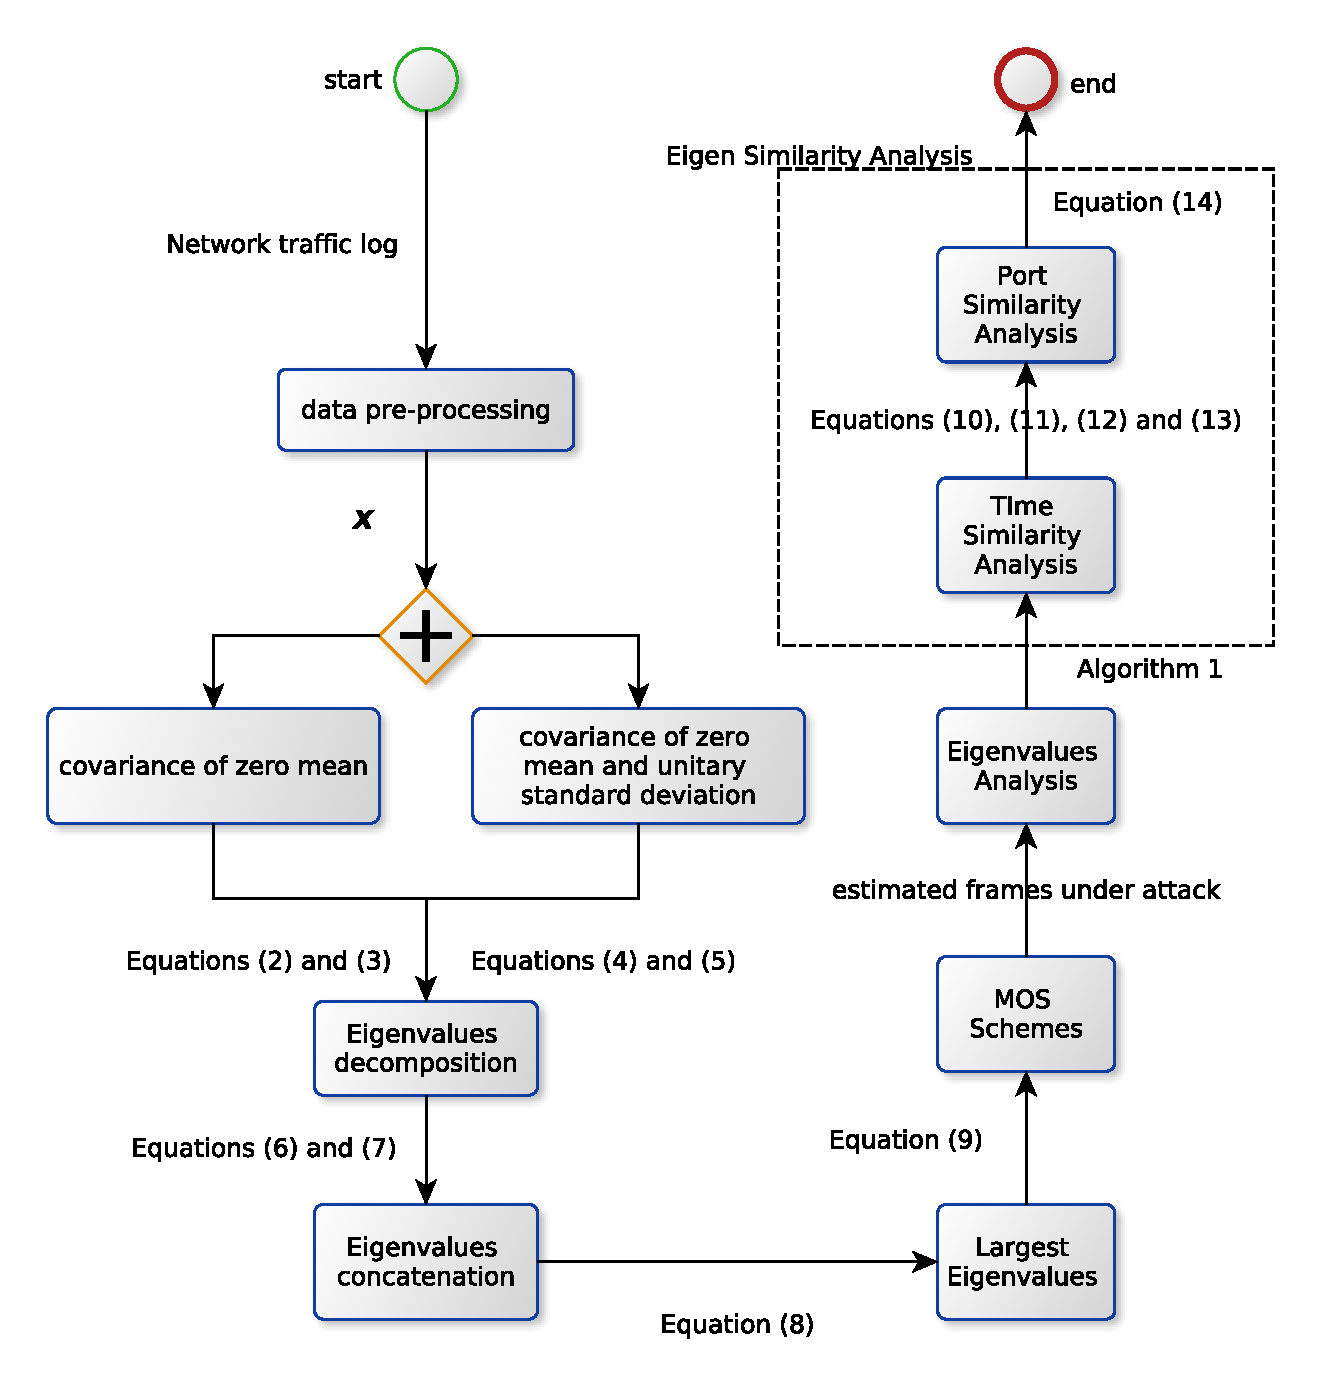
\includegraphics[width=7cm]{../figures/mos_eigen_similarity.eps}
	     \caption{Overview of The Framework for Detection and Identification of Network Attacks.}
	     \label{fig:2_fig80}
	\end{figure}

\end{frame}
%-=-=-=-=-=-=-=-=-=-=-=-=-=-=-=-=-=-=-=-=-=-=-=-=
%	FRAME: Proposed Framework
%-=-=-=-=-=-=-=-=-=-=-=-=-=-=-=-=-=-=-=-=-=-=-=-=
\begin{frame}{Proposed Framework}
	
	For flooding detection, calculate the sample covariance matrix $\boldsymbol{\hat{R}}_{yy}^{(q)}$ of the zero mean samples given by
	\begin{equation}\label{eq:eq02}
		\boldsymbol{y}_{m}^{(q)} = \boldsymbol{x}_{m}^{(q)} - \bar{\boldsymbol{x}}_{m}^{(q)}.
	\end{equation}

	the sample covariance matrix $\boldsymbol{\hat{R}}_{yy}^{(q)}$ can be calculated as follows
	\begin{equation}\label{eq:eq03}
		\boldsymbol{\hat{R}}_{yy}^{(q)} = \frac{1}{N}\boldsymbol{Y}^{(q)}\boldsymbol{Y}^{(q)^{\rm T}}.
	\end{equation}

\end{frame}
%-=-=-=-=-=-=-=-=-=-=-=-=-=-=-=-=-=-=-=-=-=-=-=-=
%	FRAME: Proposed Framework
%-=-=-=-=-=-=-=-=-=-=-=-=-=-=-=-=-=-=-=-=-=-=-=-=
\begin{frame}{Proposed Framework}
	
	For probing detection, compute the sample covariance $\boldsymbol{\hat{R}}_{zz}^{(q)}$ whose variables have zero mean and unitary standard deviation as follows
	\begin{equation}\label{eq:eq04}
		\boldsymbol{z}_{m}^{(q)} = \frac{\boldsymbol{x}_{m}^{(q)} - \bar{\boldsymbol{x}}_{m}^{(q)}}{\boldsymbol{\sigma}_{m}^{(q)}}.
	\end{equation}

	The sample covariance matrix $\boldsymbol{\hat{R}}_{zz}^{(q)}$ can be calculated via 
	\begin{equation}\label{eq:eq05}
		\boldsymbol{\hat{R}}_{zz}^{(q)} = \frac{1}{N}\boldsymbol{Z}^{(q)}\boldsymbol{Z}^{(q)^{\rm T}}.
	\end{equation}

\end{frame}
%-=-=-=-=-=-=-=-=-=-=-=-=-=-=-=-=-=-=-=-=-=-=-=-=
%	FRAME: Proposed Framework
%-=-=-=-=-=-=-=-=-=-=-=-=-=-=-=-=-=-=-=-=-=-=-=-=
\begin{frame}{Proposed Framework}
	
	we refer to $\boldsymbol{\hat{R}}_{yy}$ and $\boldsymbol{\hat{R}}_{zz}$ as a matrix $\boldsymbol{C}$

	Compute eigenvalue decomposition (EVD) to obtain the vector of eigenvalues $\boldsymbol{e}^{(q)}$ associated with each matrix, according to (\ref{eq:eq060}).
	\begin{equation}\label{eq:eq06}
	\boldsymbol{C}^{(q)} = \boldsymbol{V}^{(q)}\boldsymbol{\Lambda}^{(q)}\boldsymbol{V}^{(q)^{\rm T}},
	\end{equation}
	\begin{equation}\label{eq:eq060}
	\boldsymbol{e}^{(q)} = \rm diag(\boldsymbol{\Lambda}^{(q)}),
	\end{equation}

	The eigenvalues should be sorted in descending order, i.e., $\lambda_{1}^{(q)} > \lambda_{2}^{(q)} > \lambda_{3}^{(q)} > ... > \lambda_{m}^{(q)}$.

\end{frame}
%-=-=-=-=-=-=-=-=-=-=-=-=-=-=-=-=-=-=-=-=-=-=-=-=
%	FRAME: Proposed Framework
%-=-=-=-=-=-=-=-=-=-=-=-=-=-=-=-=-=-=-=-=-=-=-=-=
\begin{frame}{Proposed Framework}
	
	\begin{equation}\label{eq:eq07}
		\boldsymbol{E} =
		\begin{bmatrix}
			\lambda_1^{(1)} & \lambda_1^{(2)} & \lambda_1^{(3)} & \cdots & \lambda_1^{(Q)} \\
			\lambda_2^{(1)} & \lambda_2^{(2)} & \lambda_2^{(3)} & \cdots & \lambda_2^{(Q)} \\
			\lambda_3^{(1)} & \lambda_3^{(2)} & \lambda_3^{(3)} & \cdots & \lambda_3^{(Q)} \\
			\vdots & \vdots & \ddots & \vdots  \\
			\lambda_m^{(1)} & \lambda_m^{(2)} & \lambda_m^{(3)} & \cdots & \lambda_m^{(Q)} \\
		\end{bmatrix}.
	\end{equation}

	\begin{equation}\label{eq:eq08}
		\boldsymbol{e}_{\rm max} = \boldsymbol{E}\{:,1\} = [ \lambda_1^{(1)}, \lambda_1^{(2)} ... \lambda_1^{(Q)}]
	\end{equation}

\end{frame}
%-=-=-=-=-=-=-=-=-=-=-=-=-=-=-=-=-=-=-=-=-=-=-=-=
%	FRAME: MOS Scheme
%-=-=-=-=-=-=-=-=-=-=-=-=-=-=-=-=-=-=-=-=-=-=-=-=
\begin{frame}{MOS Scheme}
	
	Traditionally the MOS schemes are applied for the eigenvalues of the vector $\boldsymbol{e}^{(q)}$. 

	The proposed approach applies MOS schemes for a vector of the largest eigenvalues of each $q$-th time frame to identify variations and estimate the model order $\hat{d}$ (estimated number of time frames under attack)

	$\boldsymbol{e}_{\rm max}$ is sorted in descending order, producing $\sim\boldsymbol{e}_{\rm max}$, that is used as input parameter for MOS schemes, according to 

	$\hat{d} = \rm{MOS}(\sim\boldsymbol{e}_{\rm max})$. 

\end{frame}
%-=-=-=-=-=-=-=-=-=-=-=-=-=-=-=-=-=-=-=-=-=-=-=-=
%	FRAME: Eigen Similarity Analysis
%-=-=-=-=-=-=-=-=-=-=-=-=-=-=-=-=-=-=-=-=-=-=-=-=
\begin{frame}{Eigen Similarity Analysis}
	
	\begin{figure}[h!]
	     \centering 
	     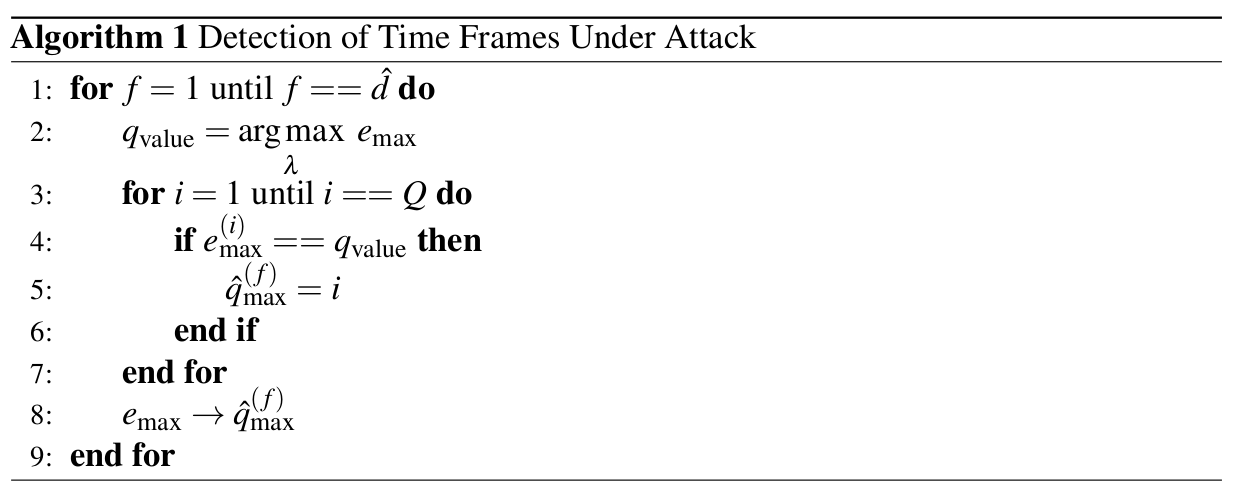
\includegraphics[width=11cm]{alg.png}
	     \label{fig:2_fig9}
	\end{figure}

\end{frame}
%-=-=-=-=-=-=-=-=-=-=-=-=-=-=-=-=-=-=-=-=-=-=-=-=
%	FRAME: Eigenvalue Analysis
%-=-=-=-=-=-=-=-=-=-=-=-=-=-=-=-=-=-=-=-=-=-=-=-=
\begin{frame}{Eigen Similarity Analysis}
	
	For eigen similarity analysis, we evaluate the cosine similarity to identify legitimate and malicious traffic,
	\begin{equation}
		\label{eq:eq11}
		s_n = \frac{\abs{\boldsymbol{v}^{(q)} \cdot \boldsymbol{v}_{(n)}}}{\norm{\boldsymbol{v}^{(q)}}\norm{\boldsymbol{v}_{(n)}}},
	\end{equation}

	$s_n$ denotes the absolute similarity degree of the $n$-th minute
	
	$\boldsymbol{v}^{(q)}$ is the most significant eigenvectors of a selected set of minutes without network attack

	$\boldsymbol{v}_{(n)}$ is the most significant eigenvectors obtained after append the target $n$-th minute of traffic to be performed the flood and port scan attack identification.

\end{frame}
%-=-=-=-=-=-=-=-=-=-=-=-=-=-=-=-=-=-=-=-=-=-=-=-=
%	FRAME: Eigenvalue Analysis
%-=-=-=-=-=-=-=-=-=-=-=-=-=-=-=-=-=-=-=-=-=-=-=-=
\begin{frame}{Eigen Similarity Analysis}
	
	The reference eigenvectors $\boldsymbol{v}^{(q)}$ is calculated from the traffic without attack. Each $\boldsymbol{x}^{(\hat{q})}_{(n)}$ vector of each $n$-th minutes of the estimated $\rm{\boldsymbol{\hat{q}}}_{\rm max}$ time frames shall be individually appended into $\boldsymbol{X}^{(q)}$, as represented by
	\begin{equation}\label{eq:eq12}
		\boldsymbol{X}_{n} = \{\boldsymbol{X}^{(q)} | \boldsymbol{x}^{(\hat{q})}_{(n)}\}.
	\end{equation}

	The resultant $\boldsymbol{X}_{(n)}$ is necessary to obtain $\boldsymbol{v}_{(n)}$, through (\ref{eq:eq06}).

\end{frame}
%-=-=-=-=-=-=-=-=-=-=-=-=-=-=-=-=-=-=-=-=-=-=-=-=
%	FRAME: Eigenvalue Analysis
%-=-=-=-=-=-=-=-=-=-=-=-=-=-=-=-=-=-=-=-=-=-=-=-=
\begin{frame}{Eigen Similarity Analysis}
	
	We evaluate three approaches for eigen similarity analysis: 
	\begin{itemize}
		\item \textbf{incremental:} concatenates eigenvectors incrementally;
		\item \textbf{individual:} concatenates each eigenvector individually and discards;
		\item \textbf{incremental individualized:} incremental until detect attach and individual after.
	\end{itemize}

\end{frame}
%-=-=-=-=-=-=-=-=-=-=-=-=-=-=-=-=-=-=-=-=-=-=-=-=
%	FRAME: Eigenvalue Analysis
%-=-=-=-=-=-=-=-=-=-=-=-=-=-=-=-=-=-=-=-=-=-=-=-=
\begin{frame}{Eigen Similarity Analysis}
	
	\begin{figure}[h!]
		\centering
	    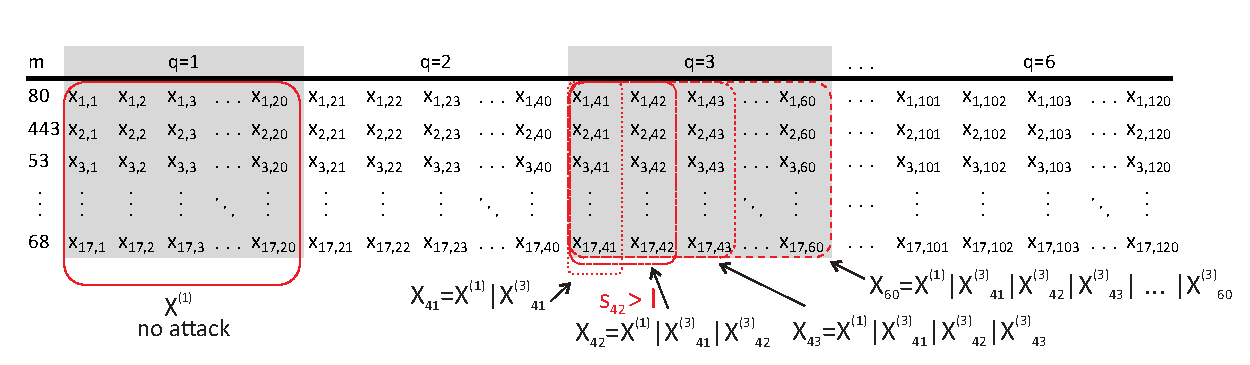
\includegraphics[width=11.5cm]{../figures/incremental.eps}
	    \caption{Traffic selection for incremental approach.}
	    \label{fig:2_fig8}
	\end{figure}

\end{frame}
%-=-=-=-=-=-=-=-=-=-=-=-=-=-=-=-=-=-=-=-=-=-=-=-=
%	FRAME: Eigenvalue Analysis
%-=-=-=-=-=-=-=-=-=-=-=-=-=-=-=-=-=-=-=-=-=-=-=-=
\begin{frame}{Eigen Similarity Analysis}
	
	\begin{figure}[h!]
	     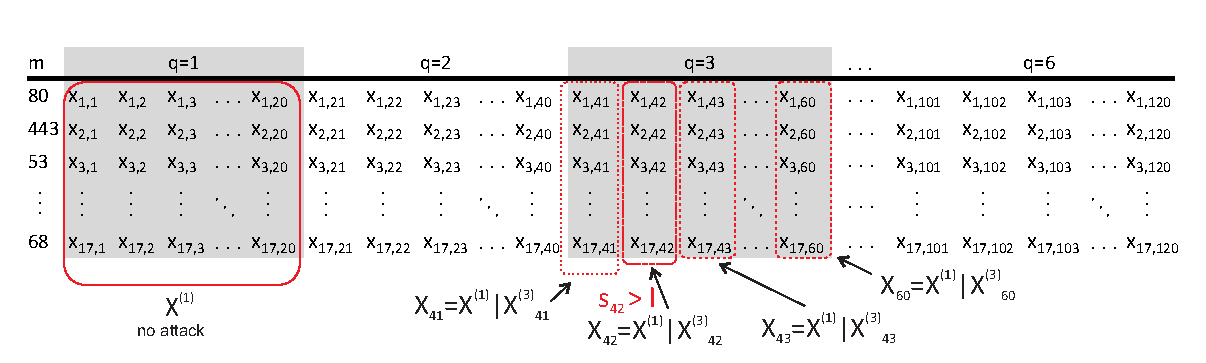
\includegraphics[width=11.5cm]{../figures/individualized.eps}
	     \caption{Traffic selection for individual approach.}
	     \label{fig:2_fig9}
	\end{figure}
\end{frame}
%-=-=-=-=-=-=-=-=-=-=-=-=-=-=-=-=-=-=-=-=-=-=-=-=
%	FRAME: Eigenvalue Analysis
%-=-=-=-=-=-=-=-=-=-=-=-=-=-=-=-=-=-=-=-=-=-=-=-=
\begin{frame}{Eigen Similarity Analysis}
	
	\begin{figure}[h!]
	     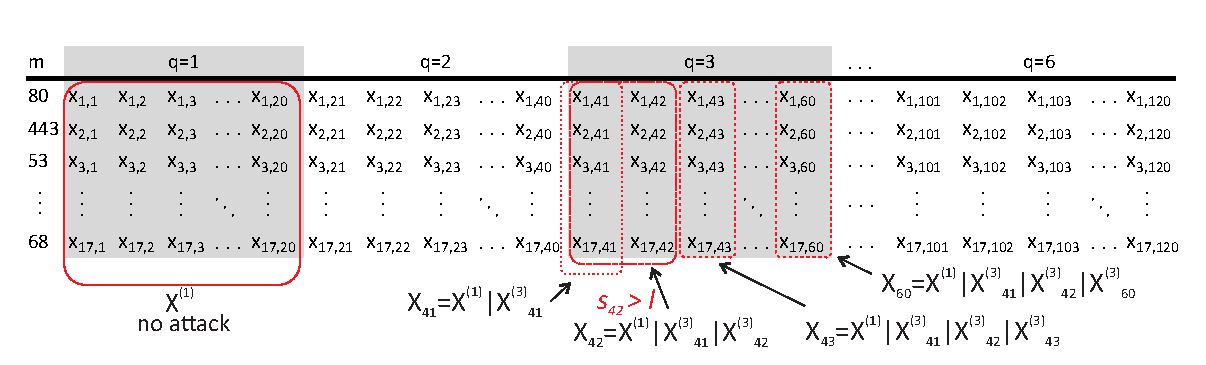
\includegraphics[width=11.5cm]{../figures/incremental_individualized.eps}
	     \caption{Traffic selection for incremental individualized approach.}
	     \label{fig:2_fig2}
	\end{figure}

\end{frame}
%-=-=-=-=-=-=-=-=-=-=-=-=-=-=-=-=-=-=-=-=-=-=-=-=
%	FRAME: Eigenvalue Analysis
%-=-=-=-=-=-=-=-=-=-=-=-=-=-=-=-=-=-=-=-=-=-=-=-=
\begin{frame}{Eigen Similarity Analysis}
	
	For detection of ports under attack, the $\boldsymbol{v}^{(q)}$ last most significant eigenvectors without attack is compared against the $\boldsymbol{v}_{(n)}$ identified as under attack, individually evaluating the cosine similarity of each $m$-th port of all $\boldsymbol{\hat{n}}$ minutes.


	\begin{equation}\label{eq:eq15}
		\left\{
		\begin{array}{@{}ll@{}}
			x_{(m,n)} = x^{(\hat{q})}_{(m,\hat{n})} \\
			\\
			s_{m,\hat{n}} = \frac{\abs{\boldsymbol{v}^{(q)} \cdot \boldsymbol{v}_{(m,\hat{n})}}}{\norm{\boldsymbol{v}^{(q)}}\norm{\boldsymbol{v}_{(m,\hat{n})}}},
		\end{array}\right.
	\end{equation}

\end{frame}
%-=-=-=-=-=-=-=-=-=-=-=-=-=-=-=-=-=-=-=-=-=-=-=-=
%	FRAME: Results
%-=-=-=-=-=-=-=-=-=-=-=-=-=-=-=-=-=-=-=-=-=-=-=-=
\begin{frame}{Results}
	
	\begin{table}[h!]
	  \centering
	  \scriptsize
	  \caption{Largest Eigenvalue related to attacks detection}
	  \label{tab:tab3}
	  \begin{tabular}{ c c c c c }
		\toprule
		\multirow{3}{*}{\textbf{Time Frame} $q$} &\multicolumn{4}{c }{\textbf{Vectors GETV}}\\ 
				\hhline{~----}
			&\textbf{Detection of}	 &\textbf{Detection of}	 &\textbf{Detection of}	 &\textbf{Detection of}\\
			&\textbf{\emph{synflood/fraggle}}	 &\textbf{\emph{synflood}}	 &\textbf{\emph{fraggle}}	 &\textbf{\emph{port scan}}\\
		\midrule
		1 &1887545 &1887545 &1887545 &2,0734 \\
		2 &2341327 &2341327 &2341327 &2,1451 \\
		3 &3213867 &3213867 &3213867 &10,0718 \\
		4 &133238294 &133238294 &731229 &2,1620 \\
		5 &92384021611 &6367983 &92384021611 &2,4253 \\
		6 &708335 &708335 &708335 &1,7948 \\
	    \bottomrule
	  \end{tabular}
	\end{table}

\end{frame}
%-=-=-=-=-=-=-=-=-=-=-=-=-=-=-=-=-=-=-=-=-=-=-=-=
%	FRAME: Results
%-=-=-=-=-=-=-=-=-=-=-=-=-=-=-=-=-=-=-=-=-=-=-=-=
\begin{frame}{Results}
	
	\begin{table}[h!]
	  \centering
	  \tiny
	  \caption{MOS schemes applied to port scan and flood detection}
	  \label{tab:tab4}
	  \begin{tabular}{ c c c c c c c c }
		\toprule
		\multirow{2}{*}{\textbf{Type of analysis} $q$} &\multicolumn{6}{c}{\textbf{MOS schemes (estimated model order $\hat{d}$)}} &{\textbf{(d)}}\\ 
				\hhline{~------~}
			&\textbf{AIC} &\textbf{MDL} &\textbf{EDC} &\textbf{RADOI} &\textbf{EFT} &\textbf{SURE}\\
		\midrule
		Detection of synflood \\(presence of attack) &2 &1 &\textbf{1} &5 &\textbf{1} &4 &\textbf{1} \\
		Detection of synflood \\(absence of attack) &1 &1 &\textbf{0} &1 &\textbf{0} &3 &\textbf{0} \\
		\midrule
		Detection of fraggle \\(presence of attack) &1 &1 &\textbf{1} &5 &\textbf{1} &4 &\textbf{1} \\
		Detection of fraggle \\(absence of attack) &1 &1 &\textbf{0} &1 &\textbf{0} &3 &\textbf{0} \\
		\midrule
		Detection of port scan \\(presence of attack) &1 &1 &\textbf{1} &1 &\textbf{1} &9 &\textbf{1} \\
		Detection of port scan \\(absence of attack) &0 &0 &\textbf{0} &1 &\textbf{0} &1 &\textbf{0} \\
		\midrule
		Detection of synflood/fraggle \\(presence of attack) &2 &2 &\textbf{2} &5 &\textbf{2} &5 &\textbf{2} \\
		Detection of synflood/fraggle \\(absence of attack) &1 &1 &\textbf{0} &1 &\textbf{0} &3 &\textbf{0} \\
	    \bottomrule
	  \end{tabular}
	\end{table}

\end{frame}
%-=-=-=-=-=-=-=-=-=-=-=-=-=-=-=-=-=-=-=-=-=-=-=-=
%	FRAME: Results
%-=-=-=-=-=-=-=-=-=-=-=-=-=-=-=-=-=-=-=-=-=-=-=-=
\begin{frame}{Results}
	
	MOS schemes for probing and flooding attack detection:
	\begin{itemize}
		\item The largest eigenvalues visually indicate the time frame under probing and flooding attack detection, but MOS schemes can estimate it mathematically;
		\item EDC and EFT estimate correctly the number of attacks $d$;
		\item EDC is the MOS scheme that requires less processing capacity.
	\end{itemize}

\end{frame}
%-=-=-=-=-=-=-=-=-=-=-=-=-=-=-=-=-=-=-=-=-=-=-=-=
%	FRAME: Results
%-=-=-=-=-=-=-=-=-=-=-=-=-=-=-=-=-=-=-=-=-=-=-=-=
\begin{frame}{Results}
	
	\begin{table}[h!]
	  \centering
	  \tiny
	  \caption{Eigen Similarity Analysis for Port Scan Detection}
	  \label{tab:tab5}
	  \begin{tabular}{ c c c c c c }
		\toprule
		\multirow{2}{*}{\textbf{Time Frame} $q$} &\multirow{2}{*}{\textbf{Time} $n$}   &\multicolumn{3}{c}{\textbf{Similarity Analysis}} &\multirow{2}{*}{\textbf{Attack?}}\\ 
				\hhline{~~---~}
				& &\textbf{Incremental Individualized} &\textbf{Incremental} &\textbf{Individual}\\
		\midrule
		3 &1 &0.9946 &0.9946 &0.9946 &no \\
		3 &2 &0.9934 &0.9934 &0.9999 &no \\
		3 &3 &0.9912 &0.9912 &0.9999 &no \\
		3 &4 &0.9888 &0.9888 &0.9999 &no \\
		3 &5 &0.9856 &0.9856 &0.9998 &no \\
		3 &6 &0.9840 &0.9840 &0.9999 &no \\
		3 &7 &0.9824 &0.9824 &1.0000 &no \\
		3 &8 &0.9794 &0.9794 &0.9999 &no \\
		3 &9 &0.9673 &0.9673 &0.9926 &no \\
		3 &10 &0.9674 &0.9674 &0.9997 &no \\
		3 &11 &0.9733 &0.9733 &0.9993 &no \\
		3 &12 &0.9702 &0.9702 &0.9993 &no \\
		3 &13 &0.9677 &0.9677 &0.9999 &no \\
		3 &14 &0.9646 &0.9646 &0.9998 &no \\
		3 &15 &0.0216 &0.0216 &0.0276 &yes \\
		3 &16 &0.9621 &0.0209 &1.0000 &no \\
		3 &17 &0.9611 &0.0199 &0.9998 &no \\
		3 &18 &0.9612 &0.0191 &0.9999 &no \\
		3 &19 &0.9613 &0.0186 &0.9998 &no \\
		3 &20 &0.9638 &0.0190 &1.0000 &no \\
	    \bottomrule
	  \end{tabular}
	\end{table}	
	
\end{frame}
%-=-=-=-=-=-=-=-=-=-=-=-=-=-=-=-=-=-=-=-=-=-=-=-=
%	FRAME: Results
%-=-=-=-=-=-=-=-=-=-=-=-=-=-=-=-=-=-=-=-=-=-=-=-=
\begin{frame}{Results}
	
	\begin{table}[h!]
	  \centering
	  \tiny
	  \caption{Eigen Similarity Analysis for Synflood Detection}
	  \label{tab:tab6}
	  \begin{tabular}{ c c c c c c }
		\toprule
		\multirow{2}{*}{\textbf{Time Frame} $q$} &\multirow{2}{*}{\textbf{Time} $n$}   &\multicolumn{3}{c}{\textbf{Similarity Analysis}} &\multirow{2}{*}{\textbf{Attack?}}\\ 
				\hhline{~~---~}
				& &\textbf{Incremental Individualized} &\textbf{Incremental} &\textbf{Individual}\\
		\midrule
		4 &1 &1.0000 &1.0000 &1.0000 &no \\
		4 &2 &0.9999 &0.9999 &1.0000 &no \\
		4 &3 &0.9997 &0.9997 &0.9999 &no \\
		4 &4 &0.9998 &0.9998 &1.0000 &no \\
		4 &5 &0.9965 &0.9965 &0.9908 &no \\
		4 &6 &0.9975 &0.9975 &1.0000 &no \\
		4 &7 &0.9977 &0.9977 &1.0000 &no \\
		4 &8 &0.9980 &0.9980 &1.0000 &no \\
		4 &9 &0.9987 &0.9987 &0.9999 &no \\
		4 &10 &0.9991 &0.9991 &1.0000 &no \\
		4 &11 &0.0085 &0.0085 &0.0284 &yes \\
		4 &12 &0.0162 &0.0120 &0.0343 &yes \\
		4 &13 &0.0248 &0.0158 &0.0427 &yes \\
		4 &14 &0.1243 &0.0185 &0.1041 &yes \\
		4 &15 &0.0082 &0.0162 &0.0103 &yes \\
		4 &16 &0.0404 &0.0070 &0.0580 &yes \\
		4 &17 &0.0397 &0.0007 &0.0573 &yes \\
		4 &18 &0.0408 &0.0042 &0.0584 &yes \\
		4 &19 &0.0408 &0.0079 &0.0584 &yes \\
		4 &20 &0.0477 &0.0092 &0.0757 &yes \\
	    \bottomrule
	  \end{tabular}
	\end{table}	
	
\end{frame}
%-=-=-=-=-=-=-=-=-=-=-=-=-=-=-=-=-=-=-=-=-=-=-=-=
%	FRAME: Results
%-=-=-=-=-=-=-=-=-=-=-=-=-=-=-=-=-=-=-=-=-=-=-=-=
\begin{frame}{Results}
	
	\begin{table}[h!]
	  \centering
	  \tiny
	  \caption{Eigen Similarity Analysis for Fraggle Detection}
	  \label{tab:tab7}
	  \begin{tabular}{ c c c c c c }
		\toprule
		\multirow{2}{*}{\textbf{Time Frame} $q$} &\multirow{2}{*}{\textbf{Time} $n$}   &\multicolumn{3}{c}{\textbf{Similarity Analysis}} &\multirow{2}{*}{\textbf{Attack?}}\\ 
				\hhline{~~---~}
				& &\textbf{Incremental Individualized} &\textbf{Incremental} &\textbf{Individual}\\
		\midrule
		5 &1 &1.0000 &1.0000 &1.0000 &no \\
		5 &2 &0.9999 &0.9999 &1.0000 &no \\
		5 &3 &1.0000 &1.0000 &1.0000 &no \\
		5 &4 &0.9999 &0.9999 &1.0000 &no \\
		5 &5 &0.9993 &0.9993 &0.9997 &no \\
		5 &6 &0.9993 &0.9993 &0.9997 &no \\
		5 &7 &0.9994 &0.9994 &1.0000 &no \\
		5 &8 &0.9995 &0.9995 &1.0000 &no \\
		5 &9 &0.9995 &0.9995 &1.0000 &no \\
		5 &10 &0.9995 &0.9995 &1.0000 &no \\
		5 &11 &0.0031 &0.0031 &0.0021 &yes \\
		5 &12 &0.0019 &0.0025 &0.0009 &yes \\
		5 &13 &0.0030 &0.0026 &0.0020 &yes \\
		5 &14 &0.0030 &0.0027 &0.0020 &yes \\
		5 &15 &0.0030 &0.0028 &0.0020 &yes \\
		5 &16 &0.0012 &0.0025 &0.0002 &yes \\
		5 &17 &0.0030 &0.0026 &0.0020 &yes \\
		5 &18 &0.0030 &0.0026 &0.0020 &yes \\
		5 &19 &0.0030 &0.0027 &0.0020 &yes \\
		5 &20 &0.0069 &0.0023 &0.0083 &yes \\
	    \bottomrule
	  \end{tabular}
	\end{table}
	
\end{frame}
%-=-=-=-=-=-=-=-=-=-=-=-=-=-=-=-=-=-=-=-=-=-=-=-=
%	FRAME: Results
%-=-=-=-=-=-=-=-=-=-=-=-=-=-=-=-=-=-=-=-=-=-=-=-=
\begin{frame}{Results}
	
	\begin{table}[h!]
	  \centering
	  \tiny
	  \caption{Eigen Similarity Analysis for Detection of Ports Under Port Scan Attack (q=3 and n=15)}
	  \label{tab:tab8}
	  \begin{tabular}{ c c c c }
		\toprule
		\multirow{2}{*}{\textbf{Port} $p$}   &\multicolumn{2}{c}{\textbf{Approaches}} &\multirow{2}{*}{\textbf{Attack?}}\\ 
				\hhline{~--~}
				&\textbf{Incremental Individualized} &\textbf{Individual}\\
		\midrule
		80 &0.9999 &0.9999 &no \\
		443 &0.9999 &0.9999 &no \\
		53 &0.9999 &0.9999 &no \\
		21 &0.9999 &0.9997 &yes \\
		22 &0.0298 &0.9997 &yes \\
		23 &0.0298 &0.9997 &yes \\
		25 &0.0298 &0.9997 &yes \\
		110 &0.0298 &0.9997 &yes \\
		143 &0.0298 &0.9997 &yes \\
		161 &0.0298 &0.9997 &yes \\
		69 &0.0298 &0.9997 &yes \\
		123 &0.0298 &0.9997 &yes \\
		445 &0.0298 &0.9997 &yes \\
		600 &0.9999 &0.9999 &no \\
		19 &0.9999 &0.9999 &no \\
		67 &0.9999 &0.9999 &no \\
		68 &0.9999 &0.9999 &no \\
	    \bottomrule
	  \end{tabular}
	\end{table}
	
\end{frame}
%-=-=-=-=-=-=-=-=-=-=-=-=-=-=-=-=-=-=-=-=-=-=-=-=
%	FRAME: Results
%-=-=-=-=-=-=-=-=-=-=-=-=-=-=-=-=-=-=-=-=-=-=-=-=
\begin{frame}{Results}
	
	\begin{table}[h!]
	  \centering
	  \tiny
	  \caption{Eigen Similarity Analysis for Detection of Ports Under Synflood Attack (q=4 and n=11)}
	  \label{tab:tab9}
	  \begin{tabular}{ c c c c }
		\toprule
		\multirow{2}{*}{\textbf{Port} $p$}   &\multicolumn{2}{c}{\textbf{Approaches}} &\multirow{2}{*}{\textbf{Attack?}}\\ 
				\hhline{~--~}
				&\textbf{Incremental Individualized} &\textbf{Individual}\\
		\midrule
		80 &1.0000 &1.0000 &no \\
		443 &1.0000 &1.0000 &no \\
		53 &1.0000 &1.0000 &no \\
		21 &1.0000 &1.0000 &nos \\
		22 &1.0000 &1.0000 &no \\
		23 &1.0000 &1.0000 &no \\
		25 &1.0000 &1.0000 &no \\
		110 &1.0000 &1.0000 &no \\
		143 &1.0000 &1.0000 &no \\
		161 &1.0000 &1.0000 &no \\
		69 &1.0000 &1.0000 &no \\
		123 &1.0000 &1.0000 &no \\
		445 &1.0000 &1.0000 &no \\
		600 &0.0077 &0.0427 &yes \\
		19 &1.0000 &1.0000 &no \\
		67 &1.0000 &1.0000 &no \\
		68 &1.0000 &1.0000 &no \\
	    \bottomrule
	  \end{tabular}
	\end{table}
	
\end{frame}
%-=-=-=-=-=-=-=-=-=-=-=-=-=-=-=-=-=-=-=-=-=-=-=-=
%	FRAME: Results
%-=-=-=-=-=-=-=-=-=-=-=-=-=-=-=-=-=-=-=-=-=-=-=-=
\begin{frame}{Results}
	
	\begin{table}[h!]
	  \centering
	  \tiny
	  \caption{Eigen Similarity Analysis for Detection of Ports Under Fraggle Attack (q=5 and t=11)}
	  \label{tab:tab10}
	  \begin{tabular}{ c c c c }
		\toprule
		\multirow{2}{*}{\textbf{Port} $p$}   &\multicolumn{2}{c}{\textbf{Approaches}} &\multirow{2}{*}{\textbf{Attack?}}\\ 
				\hhline{~--~}
				&\textbf{Incremental Individualized} &\textbf{Individual}\\
		\midrule
		80 &1.0000 &1.0000 &no \\
		443 &1.0000 &1.0000 &no \\
		53 &1.0000 &1.0000 &no \\
		21 &1.0000 &1.0000 &no \\
		22 &1.0000 &1.0000 &no \\
		23 &1.0000 &1.0000 &no \\
		25 &1.0000 &1.0000 &no \\
		110 &1.0000 &1.0000 &no \\
		143 &1.0000 &1.0000 &no \\
		161 &1.0000 &1.0000 &no \\
		69 &1.0000 &1.0000 &no \\
		123 &1.0000 &1.0000 &no \\
		445 &1.0000 &1.0000 &no \\
		600 &1.0000 &1.0000 &no \\
		19 &0.0031 &0.0004 &yes \\
		67 &1.0000 &1.0000 &no \\
		68 &1.0000 &1.0000 &no \\
	    \bottomrule
	  \end{tabular}
	\end{table}
	
\end{frame}
%-=-=-=-=-=-=-=-=-=-=-=-=-=-=-=-=-=-=-=-=-=-=-=-=
%	FRAME: Results
%-=-=-=-=-=-=-=-=-=-=-=-=-=-=-=-=-=-=-=-=-=-=-=-=
\begin{frame}{Results}
	
	For time attack detection:
	\begin{itemize}
		\item High similarity between network traffic without attack (0.9610) and low similarity with attack (0.0276);
		\item The incremental approach produces false positive results;
		\item Capability of change detection based on similarity between legitimate and malicious traffic (flood or probe);
	\end{itemize}
	
	For port attack detection:
	\begin{itemize}
		\item The incremental individualized has more sensibility to anomaly detection;
		\item The individual approach was not able to identify low similarity for ports under attack;
	\end{itemize}
	
\end{frame}
%-=-=-=-=-=-=-=-=-=-=-=-=-=-=-=-=-=-=-=-=-=-=-=-=
%	FRAME: Results
%-=-=-=-=-=-=-=-=-=-=-=-=-=-=-=-=-=-=-=-=-=-=-=-=
\begin{frame}{Results}
	
	Conclusion:
	\begin{itemize}
		\item \textbf{Incremental individualized can detect} low similarity for all evaluated network attacks, while the \textbf{other approaches presented false positives or low sensibility};
		\item This approach is able to \textbf{gradually and incrementally adapt to network traffic changing}.
	\end{itemize}

\end{frame}
%-=-=-=-=-=-=-=-=-=-=-=-=-=-=-=-=-=-=-=-=-=-=-=-=
%	FRAME: Results - DARPA Dataset
%-=-=-=-=-=-=-=-=-=-=-=-=-=-=-=-=-=-=-=-=-=-=-=-=
\begin{frame}{Results - DARPA Dataset}
	
	\begin{table}[!t]
		\caption{Results of the attack detection evaluation}
		\label{tab:tab12}
		\centering
		\scriptsize
		\begin{tabular}{|c|c|c|c|c|}
			\hline \rowcolor{Gray} \begin{tabular}[x]{@{}l@{}}Solution\end{tabular}	& \begin{tabular}[x]{@{}l@{}}Attack Type\end{tabular}	 & \begin{tabular}[x]{@{}l@{}}Metric\end{tabular}	& \begin{tabular}[x]{@{}l@{}}Result\end{tabular} \\ \hline
			Proposed Work	&Flooding	&True Positive	&100.00 \%\\ \hline
			Proposed Work	&Flooding	&False Positive	&60.00 \%\\ \hline
			Proposed Work	&Flooding	&Misclassification	&50.00 \%\\ \hline
			Proposed Work	&Probe	&True Positive	&76.92 \%\\ \hline
			Proposed Work	&Probe	&False Positive	&18.52 \%\\ \hline
			Proposed Work	&Probe	&Misclassification	&32.73 \%\\ \hline
			Callegari \emph{et al}	&Flooding	&True Positive	&82.00 \%\\ \hline
			Callegari \emph{et al}	&Flooding	&False Positive	&-\\ \hline
			Callegari \emph{et al}	&Flooding	&Misclassification	&-\\ \hline
			Lu and Ghorbani	&Overall	&True Positive	&94.67 \%\\ \hline
			Lu and Ghorbani	&Overall	&False Positive	&-\\ \hline
			Lu and Ghorbani	&Overall	&Misclassification	&-\\ \hline
			Lu and Ghorbani	&Portsweep	&True Positive	&50.00 \%\\ \hline
			Lu and Ghorbani	&Portsweep	&False Positive	&-\\ \hline
			Lu and Ghorbani	&Portsweep	&Misclassification	&-\\ \hline
		\end{tabular}
	\end{table}
	
\end{frame}
%-=-=-=-=-=-=-=-=-=-=-=-=-=-=-=-=-=-=-=-=-=-=-=-=
%	FRAME: Results - DARPA Dataset
%-=-=-=-=-=-=-=-=-=-=-=-=-=-=-=-=-=-=-=-=-=-=-=-=
\begin{frame}{Results - DARPA Dataset}
	
	Misclassification is defined as $\frac{(FN+FP)}{(TP+FP+FN+TN)}$;

	High FP and misclassification due to legitimate traffic be massive (such as an attack) sometimes;

	Callegari \emph{et al} is a statistical method, based on PCA, without training or learning methods
	\begin{itemize}
		\item 82 \% while we obtain 100 \%;
		\item FP and misclassification was not evaluated.
	\end{itemize}

	Ghorbani's is based on signal processing techniques and uses DARPA
	\begin{itemize}
		\item 94.67 \% and 50.00 \%, while we obtain 100 \% and 76.92 \%;
		\item FP and misclassification was not evaluated.
	\end{itemize}

\end{frame}
%-=-=-=-=-=-=-=-=-=-=-=-=-=-=-=-=-=-=-=-=-=-=-=-=
%	FRAME: Performance Evaluation
%-=-=-=-=-=-=-=-=-=-=-=-=-=-=-=-=-=-=-=-=-=-=-=-=
\begin{frame}{Performance Evaluation}

	Complexity Analysis:
	\begin{itemize}
		\item the proposed framework is $O(N^3 + Q \log Q + \hat{d}Q + N^3)$ and its worst-case running time is $O(N^3)$;
		\item The computational complexity of EVD is predominant in the framework;
		\item However, the approach splits the data into time frames with period time $N$, which makes possible to limit the growth of $N$ even for evaluations of cases with total time larger than $N$;
		\item It reduces the impact caused by the computational complexity of EVD.
	\end{itemize}
	
\end{frame}
%-=-=-=-=-=-=-=-=-=-=-=-=-=-=-=-=-=-=-=-=-=-=-=-=
%	FRAME: Performance Evaluation
%-=-=-=-=-=-=-=-=-=-=-=-=-=-=-=-=-=-=-=-=-=-=-=-=
\begin{frame}{Performance Evaluation}
	
	Processing Time Analysis:
	\begin{itemize}
		\item desktop computer with a Intel Core i7-4510U 2.00GHz and 16 GB of RAM;
		\item variations on the network traffic time; 
		\item the frame size denoted as $N$; 
		\item the number of network ports denoted as $M$; 
		\item the mean processing time for eigen analysis based on sample covariance of zero mean (1-time); 
		\item the mean processing time for eigen analysis based on sample covariance of zero mean and unitary standard deviation (2-time); 
		\item the mean processing time for EDC MOS scheme, (3-time).
	\end{itemize}
	
\end{frame}
%-=-=-=-=-=-=-=-=-=-=-=-=-=-=-=-=-=-=-=-=-=-=-=-=
%	FRAME: Performance Evaluation
%-=-=-=-=-=-=-=-=-=-=-=-=-=-=-=-=-=-=-=-=-=-=-=-=
\begin{frame}{Performance Evaluation}
	
	\begin{table}[!t]
		\caption{Processing time of the main steps for anomaly detection}
		\label{tab:11}
		\centering
		\tiny
		\begin{tabular}{|r|r|r|r|r|r|r|}
			\hline \rowcolor{Gray} \begin{tabular}[x]{@{}l@{}}Traffic Time\\(hour)\end{tabular}	& \begin{tabular}[x]{@{}l@{}}Frame Size\\(min)\end{tabular}	 & \begin{tabular}[x]{@{}l@{}}Num. Ports\end{tabular}	& \begin{tabular}[x]{@{}l@{}}1-time\\(ms)\end{tabular}	& \begin{tabular}[x]{@{}l@{}}2-time\\(ms)\end{tabular}	& \begin{tabular}[x]{@{}l@{}}3-time\\(ms)\end{tabular}	\\ \hline
			16	& 10	& 17	& 0.7900	& 0.8100	& 0.0650\\ \hline
			16	& 20	& 17	& 0.5250	& 0.5950	& 0.0100\\ \hline
			16	& 60	& 17	& 0.9700	& 1.1400	& 0.0250\\ \hline
			16	& 120	& 17	& 0.6050	& 0.6100	& 0.0050\\ \hline
			16	& 60	& 34	& 1.2750	& 1.2200	& 0.0050\\ \hline
			16	& 120	& 34	& 1.1200	& 1.1700	& 0.0050\\ \hline
			20	& 10	& 17	& 2.7950	& 2.8950	& 1.1000\\ \hline
			20	& 20	& 17	& 2.0700	& 2.0200	& 0.3500\\ \hline
			20	& 60	& 17	& 1.0250	& 1.0450	& 0.0650\\ \hline
			20	& 120	& 17	& 1.0000	& 1.0700	& 0.0350\\ \hline
			20	& 60	& 34	& 2.9650	& 3.2100	& 0.0400\\ \hline
			20	& 120	& 34	& 2.9950	& 3.1150	& 0.0200\\ \hline
			22	& 10	& 17	& 4.7250	& 4.0850	& 1.4600\\ \hline
			22	& 20	& 17	& 2.3200	& 2.6800	& 0.2450\\ \hline
			22	& 60	& 17	& 1.0700	& 1.1200	& 0.0300\\ \hline
			22	& 120	& 17	& 0.9900	& 1.0500	& 0.0250\\ \hline
			22	& 60	& 34	& 3.0850	& 3.1250	& 0.0650\\ \hline
			22	& 120	& 34	& 2.8100	& 2.9600	& 0.0250\\ \hline
		\end{tabular}
	\end{table}
	
\end{frame}
%-=-=-=-=-=-=-=-=-=-=-=-=-=-=-=-=-=-=-=-=-=-=-=-=
%	FRAME: Performance Evaluation
%-=-=-=-=-=-=-=-=-=-=-=-=-=-=-=-=-=-=-=-=-=-=-=-=
\begin{frame}{Performance Evaluation}

	Processing Time Analysis:
	\begin{itemize}
		\item The processing time increases according to the increment in traffic time, around 2 or 3 times for 1-time and 2-time, but the worst measured processing time is 4.7250 milliseconds;
		\item the processing time increases with the frame size $N$ decreasing;
		\item The number of ports evaluated during the proposed scheme is also an important variable regarding processing time optimizations.
	\end{itemize}
	
\end{frame}



























%-=-=-=-=-=-=-=-=-=-=-=-=-=-=-=-=-=-=-=-=-=-=-=-=
%	SECTION: Offline Mode for Corporate Mobile Client Security Architecture
%-=-=-=-=-=-=-=-=-=-=-=-=-=-=-=-=-=-=-=-=-=-=-=-=
\section{Offline Mode for Corporate Mobile Client Security Architecture}
\label{Blocks}
%-=-=-=-=-=-=-=-=-=-=-=-=-=-=-=-=-=-=-=-=-=-=-=-=
%	FRAME: Blocks
%-=-=-=-=-=-=-=-=-=-=-=-=-=-=-=-=-=-=-=-=-=-=-=-=

\begin{frame}{Blocks}

\begin{block}{Block Title Here}
		Great for definitions
\end{block}

\begin{alertblock}{Alert Title Here}
		Great for definitions
\end{alertblock}

\begin{exampleblock}{Example Title Here}
		Great for examples
\end{exampleblock}
\end{frame}

%-=-=-=-=-=-=-=-=-=-=-=-=-=-=-=-=-=-=-=-=-=-=-=-=
%	FRAME: Blocks
%-=-=-=-=-=-=-=-=-=-=-=-=-=-=-=-=-=-=-=-=-=-=-=-=

\begin{frame}{Blocks}

\begin{block}{Block Title Here}
	\begin{itemize}
		\item point 1
		\item point 2
	\end{itemize}
\end{block}

\begingroup
\setbeamercolor{block title}{fg=white, bg=\cnBlue}
\setbeamercolor{block body}{bg=\cnLightBlue}
\begin{block}{Blue Colored Blocks}
	Produced by using the \texttt{cblock} theme option
\end{block}
\endgroup
\end{frame}

%-=-=-=-=-=-=-=-=-=-=-=-=-=-=-=-=-=-=-=-=-=-=-=-=
%	FRAME: Additional Blocks
%-=-=-=-=-=-=-=-=-=-=-=-=-=-=-=-=-=-=-=-=-=-=-=-=

\begin{frame}{Additional Blocks}
\begin{alertblock}{Alert Block}
	Highlight important information.
\end{alertblock}

\begingroup
\setbeamercolor{block title}{fg=white, bg=\cnRed}
\setbeamercolor{block body}{bg=\cnLightRed}
\begin{block}{Red Colored Blocks}
	Produced by using the \texttt{cblock} theme option
\end{block}
\endgroup
\end{frame}

%-=-=-=-=-=-=-=-=-=-=-=-=-=-=-=-=-=-=-=-=-=-=-=-=
%	FRAME: Additional Blocks
%-=-=-=-=-=-=-=-=-=-=-=-=-=-=-=-=-=-=-=-=-=-=-=-=

\begin{frame}{Additional Blocks}

\begin{exampleblock}{Example Block}
	Examples can be good.
\end{exampleblock}

\begingroup
\setbeamercolor{block title}{fg=white, bg=\cnGreen}
\setbeamercolor{block body}{bg=\cnLightGreen}
\begin{block}{Green Colored Blocks}
	Produced by using the \texttt{cblock} theme option
\end{block}
\endgroup

\end{frame}

%-=-=-=-=-=-=-=-=-=-=-=-=-=-=-=-=-=-=-=-=-=-=-=-=
%	FRAME: Blocks
%-=-=-=-=-=-=-=-=-=-=-=-=-=-=-=-=-=-=-=-=-=-=-=-=

\begin{frame}{Custom Blocks}
\begingroup
\setbeamercolor{block title}{fg=white, bg=\cnPurple}
\setbeamercolor{block body}{bg=\cnLightPurple}
\begin{block}{Purple customization}
	Using the theme colors to generate colored blocks.
\end{block}
\endgroup

\end{frame}

%-=-=-=-=-=-=-=-=-=-=-=-=-=-=-=-=-=-=-=-=-=-=-=-=
%
%	SECTION: Tensor-based Discriminative Sensing for Fraud Detection
%
%-=-=-=-=-=-=-=-=-=-=-=-=-=-=-=-=-=-=-=-=-=-=-=-=
\section{Tensor-based Discriminative Sensing for Fraud Detection}

%-=-=-=-=-=-=-=-=-=-=-=-=-=-=-=-=-=-=-=-=-=-=-=-=
%	FRAME: 
%-=-=-=-=-=-=-=-=-=-=-=-=-=-=-=-=-=-=-=-=-=-=-=-=

\begin{frame}[c]{No Special Fonts Required}

This theme was originally made to work with \texttt{pdflatex} and the default latex fonts.\\
\vspace{1em}
\cRed{sthlm} does comes with a \texttt{pdflatex} font option, \cRed{newPxFont}, which loads the following fonts:

\begin{itemize}
	\item \emph{newpxtext} for text
	\item \emph{cantarell} for sans-serif
	\item \emph{inconsolata} for sans-serif monospaced
	\item \emph{newpxmath} for math
\end{itemize}

Please refer to the \texttt{beamerfontthememsthlm.sty} for the package requirements.

\end{frame}


%-=-=-=-=-=-=-=-=-=-=-=-=-=-=-=-=-=-=-=-=-=-=-=-=
%
%	SECTION: Conclusion and Future Work
%
%-=-=-=-=-=-=-=-=-=-=-=-=-=-=-=-=-=-=-=-=-=-=-=-=
\section{Conclusion and Future Work}

%-=-=-=-=-=-=-=-=-=-=-=-=-=-=-=-=-=-=-=-=-=-=-=-=
%	FRAME: Tables
%-=-=-=-=-=-=-=-=-=-=-=-=-=-=-=-=-=-=-=-=-=-=-=-=

\begin{frame}{Tables}
\begin{table}[]
	\caption{Selection of window function and their properties}
	\begin{tabular}[]{lrrr}
		\toprule
		\textbf{Window}			& \multicolumn{1}{c}{\textbf{First side lobe}}
		                    & \multicolumn{1}{c}{\textbf{3\,dB bandwidth}}
		                    & \multicolumn{1}{c}{\textbf{Roll-off}} \\
		\midrule
		Rectangular				& 13.2\,dB	& 0.886\,Hz/bin	& 6\,dB/oct		\\[0.25em]
		Triangular				& 26.4\,dB	& 1.276\,Hz/bin	& 12\,dB/oct	\\[0.25em]
		Hann					& 31.0\,dB	& 1.442\,Hz/bin	& 18\,dB/oct	\\[0.25em]
		Hamming					& 41.0\,dB	& 1.300\,Hz/bin	& 6\,dB/oct		\\
		\bottomrule
	\end{tabular}
	\label{tab:WindowFunctions}
\end{table}
\end{frame}

%-=-=-=-=-=-=-=-=-=-=-=-=-=-=-=-=-=-=-=-=-=-=-=-=
%	FRAME:
%-=-=-=-=-=-=-=-=-=-=-=-=-=-=-=-=-=-=-=-=-=-=-=-=

\begin{frame}[c]{Mathematics Step by Step}
Show $[x^n]'=nx^{n-1}$ by using first principles.
\begin{align*}
\visible<+->{f'(x) & = \displaystyle \lim_{\Delta x \to 0} \frac{f(x+\Delta x)-f(x)}{\Delta x} \\}
\visible<+->{&= \displaystyle \lim_{\Delta x \to 0} \frac{(\cRed{x+\Delta x})^n - (\cRed{x})^n}{\Delta x}\\}
\visible<+->{&= \displaystyle \lim_{\Delta x \to 0} \frac{\binom{n}{0}x^n\Delta x^0 +\binom{n}{1}x^{n-1}\Delta x^1 + \cdots + \binom{n}{n}x^0\Delta x^n - \cRed{x^n} }{\Delta x}\\}
\visible<+->{&= \displaystyle \lim_{\Delta x \to 0} \frac{\cRed{1}x^n(\cRed{1}) +\cRed{n}x^{n-1}\Delta x^1 + \cdots + \cRed{1}(\cRed{1})\Delta x^n - \cRed{x^n} }{\Delta x}\\}
\visible<+->{&= \displaystyle \lim_{\Delta x \to 0} \frac{\cRed{x^n} +nx^{n-1}\Delta x + \cdots + \Delta x^n - \cRed{x^n} }{\Delta x}\\}
\visible<+->{&= \displaystyle \lim_{\Delta x \to 0} \frac{\cancel{\cRed{\Delta x}} (nx^{n-1} + \cdots + \Delta x^{n-1} ) }{\cancel{\Delta x}}\\}
\visible<+->{&=nx^{n-1}}
\end{align*}

\end{frame}

%-=-=-=-=-=-=-=-=-=-=-=-=-=-=-=-=-=-=-=-=-=-=-=-=
%	FRAME: Formulas
%-=-=-=-=-=-=-=-=-=-=-=-=-=-=-=-=-=-=-=-=-=-=-=-=

\begin{frame}{Functions}
\begin{block}{Gaussian Probability Density Function}
\[
f \left(x \mid \mu, \sigma^2 \right) = \dfrac{1}{\sqrt{2 \sigma^2 \pi}} e^{- \dfrac{(x-\mu)^2}{2\sigma^2}}
\]
\end{block}
\end{frame}

%-=-=-=-=-=-=-=-=-=-=-=-=-=-=-=-=-=-=-=-=-=-=-=-=
%	FRAME: 
%-=-=-=-=-=-=-=-=-=-=-=-=-=-=-=-=-=-=-=-=-=-=-=-=

\begin{frame}[c]{More Mathematics}

\begin{columns}[c]
\begin{column}{0.5\textwidth}
\begin{tikzpicture}[scale=0.7]
	\begin{axis}[
            domain=0:2, range=0:6,ymax=6,ymin=0,
            axis lines =left,
            every axis y label/.style={at=(current axis.above origin),anchor=south},
            every axis x label/.style={at=(current axis.right of origin),anchor=west},
            xtick={1,1.666}, ytick={1,3},
            xticklabels={$\cPurple{x}$,$\cPurple{x}+\cRed{\Delta x}$}, yticklabels={$f(\cPurple{x})$,$f(\cPurple{x}+\cRed{\Delta x})$},
            axis on top,
          ]
          \addplot [very thick,\cnRed, domain=(0:2)] {-1.994+2.994*x};S
	  	  \addplot [\cnDarkGrey,dashed] plot coordinates {(1,0) (1,1)};
          \addplot [\cnDarkGrey,dashed] plot coordinates {(0,1) (1,1)};
          \addplot [\cnDarkGrey,dashed] plot coordinates {(0,3) (1.666,3)};
          \addplot [\cnDarkGrey,dashed] plot coordinates {(1.666,0) (1.666,3)};
          \addplot [very thick,\cnBlue, smooth,domain=(0:1.833)] {-1/(x-2)};
          \addplot[color=\cnDarkGrey,fill=\cnDarkGrey,only marks,mark=*] coordinates{(1.666,3)};  %% closed hole
          \addplot[color=\cnDarkGrey,fill=\cnDarkGrey,only marks,mark=*] coordinates{(1,1)};  %% closed hole
        \end{axis}
\end{tikzpicture}
\end{column}

\begin{column}{0.5\textwidth}
\begin{align*}
m &= \frac{\Delta y}{\Delta x}	\\
\\
m & =  \frac{\visible<2->{f(\cPurple{x}+\cRed{\Delta x})}\visible<3->{-}\visible<4->{f(\cPurple{x})}}{\visible<5->{\cPurple{x}+\cRed{\Delta x}}\visible<6->{-}\visible<7->{\cPurple{x}}}\\
m  &=  \underbrace{\frac{\visible<8->{f(\cPurple{x}+\cRed{\Delta x})-f(\cPurple{x})}}{\visible<9->{\cRed{\Delta x}}}}_{\visible<10->{\text{\cRed{difference quotient}}}}
\end{align*}
\end{column}
\end{columns}

\visible<10->{The slope of the secant line }
\begin{itemize}
	\item<10-> can be found using the \cRed{difference quotient}
	\item<11-> represents a \cBlue{function}'s \cRed{average} slope on the interval $[\cPurple{x}, \cRed{x+\Delta x}]$
\end{itemize}

\end{frame}

%-=-=-=-=-=-=-=-=-=-=-=-=-=-=-=-=-=-=-=-=-=-=-=-=
%	FRAME:
%-=-=-=-=-=-=-=-=-=-=-=-=-=-=-=-=-=-=-=-=-=-=-=-=

\begin{frame}[c, fragile]{Fragile Frames Not a Problem}
\begin{tikzpicture}
	\begin{axis}[
            domain=0:6, range=0:7,
            ymin=-.2,ymax=7,
            width=\textwidth,
            height=7cm, %% Hard coded height! Moreover this effects the aspect ratio of the zoom--sort of BAD
            axis lines=none,
          ]
          \only<3->{\addplot [draw=none, fill=\cnDarkGrey!10!\cnGrey] plot coordinates {(.8,1.6) (2.834,5)} \closedcycle; %% zoom fill
          \addplot [draw=none, fill=\cnDarkGrey!10!\cnGrey] plot coordinates {(2.834,5) (4.166,5)} \closedcycle; %% zoom fill
          \addplot [draw=none, fill=white] plot coordinates {(1.2,1.6) (4.166,5)} \closedcycle; %% zoom fill
          \addplot [draw=none, fill=white] plot coordinates {(.8,1.6) (1.2,1.6)} \closedcycle; %% zoom fill
		  }
          \only<4->{\addplot [draw=none, fill=\cnDarkGrey!10!\cnGrey] plot coordinates {(3.3,3.6) (5.334,5)} \closedcycle; %% zoom fill
          \addplot [draw=none, fill=\cnDarkGrey!10!\cnGrey] plot coordinates {(5.334,5) (6.666,5)} \closedcycle; %% zoom fill
          \addplot [draw=none, fill=white] plot coordinates {(3.7,3.6) (6.666,5)} \closedcycle; %% zoom fill
          \addplot [draw=none, fill=white] plot coordinates {(3.3,3.6) (3.7,3.6)} \closedcycle; %% zoom fill
  }
          \only<4->{\addplot [draw=none, fill=\cnDarkGrey!10!\cnGrey] plot coordinates {(3.7,2.4) (6.666,1)} \closedcycle; %% zoom fill
          \addplot [draw=none, fill=\cnDarkGrey!10!\cnGrey] plot coordinates {(3.3,2.4) (3.7,2.4)} \closedcycle; %% zoom fill
          \addplot [draw=none, fill=white] plot coordinates {(3.3,2.4) (5.334,1)} \closedcycle; %% zoom fill
          \addplot [draw=none, fill=white] plot coordinates {(5.334,1) (6.666,1)} \closedcycle; %% zoom fill
 }

          \only<3->{\addplot [draw=none, fill=\cnDarkGrey!10!\cnGrey] plot coordinates {(.8,.4) (2.834,1)} \closedcycle; %% zoom fill
          \addplot [draw=none, fill=\cnDarkGrey!10!\cnGrey] plot coordinates {(2.834,1) (4.166,1)} \closedcycle; %% zoom fill
          \addplot [draw=none, fill=white] plot coordinates {(1.2,.4) (4.166,1)} \closedcycle; %% zoom fill
          \addplot [draw=none, fill=white] plot coordinates {(.8,.4) (1.2,.4)} \closedcycle; %% zoom fill
}
          \addplot[very thick,\cnRed, smooth,domain=(0:1.833)] {-1/(x-2)};
          \only<3->{\addplot[very thick,\cnRed, smooth,domain=(2.834:4.166)] {3.333/(2.050-.3*x)-0.333}; %% 2.5 to 4.333
          %\addplot[very thick,\cnRed, smooth,domain=(5.334:6.666)] {11.11/(1.540-.09*x)-8.109}; %% 5 to 6.833
          \only<4->\addplot[very thick,\cnRed, smooth,domain=(5.334:6.666)] {x-3}; %% 5 to 6.833
 }
         \only<2->{ \addplot[color=\cnRed,fill=\cnRed,only marks,mark=*] coordinates{(1,1)};}  %% point to be zoomed
          \only<3->{\addplot[color=\cnRed,fill=\cnRed,only marks,mark=*] coordinates{(3.5,3)}; } %% zoomed pt 1
          \only<4->{\addplot[color=\cnRed,fill=\cnRed,only marks,mark=*] coordinates{(6,3)}; } %% zoomed pt 2

          \addplot [->,\cnDarkGrey] plot coordinates {(0,0) (0,6)}; %% axis
          \addplot [->,\cnDarkGrey] plot coordinates {(0,0) (2,0)}; %% axis

          \only<2->{\addplot [\cnDarkGrey!50!\cnGrey] plot coordinates {(.8,.4) (.8,1.6)}; %% box around pt
          \addplot [\cnDarkGrey!50!\cnGrey] plot coordinates {(1.2,.4) (1.2,1.6)}; %% box around pt
          \addplot [\cnDarkGrey!50!\cnGrey] plot coordinates {(.8,1.6) (1.2,1.6)}; %% box around pt
          \addplot [\cnDarkGrey!50!\cnGrey] plot coordinates {(.8,.4) (1.2,.4)}; %% box around pt
 }
          \only<3->{\addplot [\cnDarkGrey!50!\cnGrey] plot coordinates {(2.834,1) (2.834,5)}; %% zoomed box 1
          \addplot [\cnDarkGrey!50!\cnGrey] plot coordinates {(4.166,1) (4.166,5)}; %% zoomed box 1
          \addplot [\cnDarkGrey!50!\cnGrey] plot coordinates {(2.834,1) (4.166,1)}; %% zoomed box 1
          \addplot [\cnDarkGrey!50!\cnGrey] plot coordinates {(2.834,5) (4.166,5)}; %% zoomed box 1
}
          \only<4->{\addplot [\cnDarkGrey] plot coordinates {(3.3,2.4) (3.3,3.6)}; %% box around zoomed pt
          \addplot [\cnDarkGrey] plot coordinates {(3.7,2.4) (3.7,3.6)}; %% box around zoomed pt
          \addplot [\cnDarkGrey] plot coordinates {(3.3,3.6) (3.7,3.6)}; %% box around zoomed pt
          \addplot [\cnDarkGrey] plot coordinates {(3.3,2.4) (3.7,2.4)}; %% box around zoomed pt
}
          \only<4->{\addplot [\cnDarkGrey] plot coordinates {(5.334,1) (5.334,5)}; %% zoomed box 2
          \addplot [\cnDarkGrey] plot coordinates {(6.666,1) (6.666,5)}; %% zoomed box 2
          \addplot [\cnDarkGrey] plot coordinates {(5.334,1) (6.666,1)}; %% zoomed box 2
          \addplot [\cnDarkGrey] plot coordinates {(5.334,5) (6.666,5)}; %% zoomed box 2
}
          \node at (axis cs:2.4,0) [anchor=east] {$x$};
          \node at (axis cs:0,6.9) [anchor=north] {$y$};
        \end{axis}
\end{tikzpicture}
\end{frame}

%-=-=-=-=-=-=-=-=-=-=-=-=-=-=-=-=-=-=-=-=-=-=-=-=
%	FRAME: PGFPlots
%-=-=-=-=-=-=-=-=-=-=-=-=-=-=-=-=-=-=-=-=-=-=-=-=

\begin{frame}{PGFPlots Example}
	\begin{figure}[h]
		\centering
		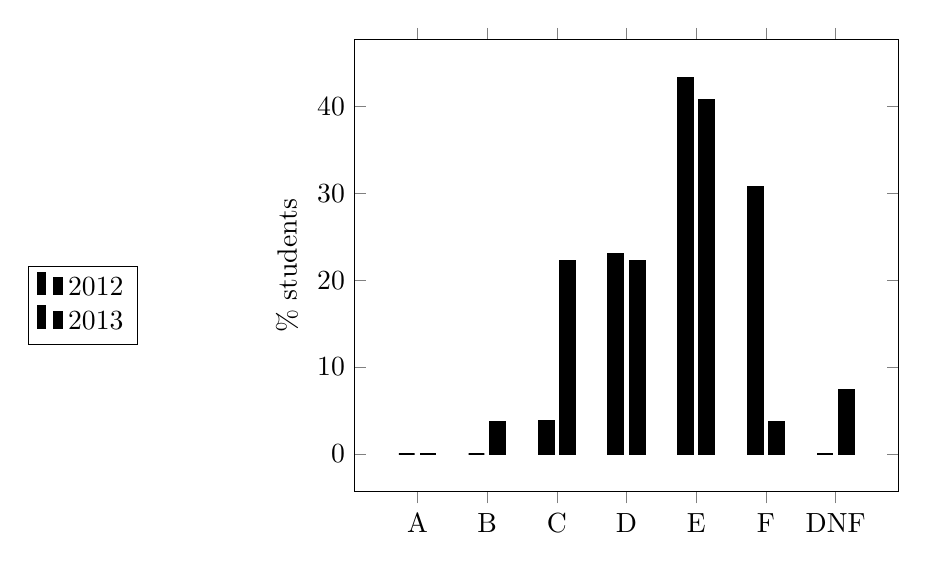
\begin{tikzpicture}
		\begin{axis}[
		    ybar,
		    enlarge x limits=0.15,
		    legend style={at={(-.5,0.5)},
		      anchor=north,legend columns=1},
		    ylabel={\% students},
		    symbolic x coords={A, B, C, D, E, F, DNF},
		    xtick=data,
		     bar width=2mm,
		     width=0.7\textwidth
		    ]
		    \legend{2012, 2013};
		    % Spring 2012 results
			\addplot[fill=\cnGrey]  coordinates {(A,0) (B,0) (C,3.85) (D,23.07) (E,43.31) (F,30.77) (DNF,0.00)};
			% Spring 2013 results
			\addplot[fill=\cnBlue]   coordinates {(A,0) (B,3.70) (C,22.22) (D,22.22) (E,40.74) (F,3.70) (DNF,7.41)};
		\end{axis}
		\end{tikzpicture}
		\caption{Consistent improvement over the last year}
		\end{figure}
\end{frame}

%-=-=-=-=-=-=-=-=-=-=-=-=-=-=-=-=-=-=-=-=-=-=-=-=
%	FRAME: Multiple Columns
%-=-=-=-=-=-=-=-=-=-=-=-=-=-=-=-=-=-=-=-=-=-=-=-=

\begin{frame}{Multiple Columns}
\begin{columns}
\begin{column}{.48\linewidth}
		Lorem ipsum dolor sit amet, consectetur adipisicing elit, sed do eiusmod
		tempor incididunt ut labore et dolore magna aliqua. Ut enim ad minim veniam.
\end{column}
\begin{column}{.48\linewidth}
		\begin{itemize}
        	\item Point 1
			\begin{itemize}
				\item Sub point a
				\item Sub point b
			\end{itemize}
        	\item Point 2
		\end{itemize}
	\end{column}
	\end{columns}
\end{frame}

\begin{frame}{References}
	\begin{thebibliography}{10}

	\beamertemplatebookbibitems
	\bibitem{Oppenheim2009}
	Alan V. Oppenheim
	\newblock Discrete - Time Signal Processing
	\newblock Prentice Hall Press, 2009

	\beamertemplatearticlebibitems
	\bibitem{EBU2011}
	European Broadcasting Union
	\newblock Specification of the Broadcast Wave Format (BWF)
	\newblock 2011

  \end{thebibliography}
\end{frame}

%-=-=-=-=-=-=-=-=-=-=-=-=-=-=-=-=-=-=-=-=-=-=-=-=
%
%	SECTION: Conclusion
%
%-=-=-=-=-=-=-=-=-=-=-=-=-=-=-=-=-=-=-=-=-=-=-=-=

\begin{frame}{About}

This sthlm beamer theme is free software: you can redistribute it and/or modify
it under the terms of the GNU General Public License as published by
the Free Software Foundation, either version 3 of the License, or
(at your option) any later version.\\
\vspace{1cm}
If you have any questions or comments
\begin{itemize}
	\item Website: \cBlue{markolson.se}
	\item Twitter: \cBlue{@markolsonse}
	\item Instagram: \cBlue{@markolson.se}
\end{itemize}
\end{frame}

%-=-=-=-=-=-=-=-=-=-=-=-=-=-=-=-=-=-=-=-=-=-=-=-=
%	FRAME:
%-=-=-=-=-=-=-=-=-=-=-=-=-=-=-=-=-=-=-=-=-=-=-=-=
\begingroup
\setbeamercolor{background canvas}{bg=\cnDarkGrey}
\begin{frame}[plain]

\centering{\cGrey{\Huge{THE \newline END}}}

\end{frame}
\endgroup

\end{document}